\documentclass[11pt,a4paper]{article}
\usepackage[utf8]{inputenc}
\usepackage[spanish]{babel}
\usepackage{amsmath}
\usepackage{amsfonts}
\usepackage{amssymb}
\usepackage{graphicx}
\usepackage{caption}
\captionsetup[table]{name=Tabla}
\date{}
\usepackage{float}
\usepackage[left=2cm,right=2cm,top=2cm,bottom=2cm]{geometry}
\title{Elección de centros}
\begin{document}
\textbf{Primer ejemplo: EDP 1}
\begin{figure}[H]
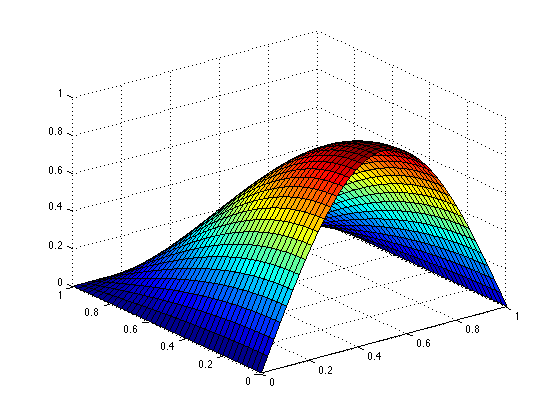
\includegraphics[scale=.5]{edp1.png}
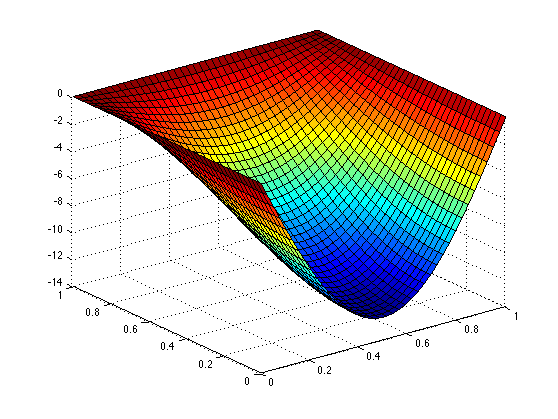
\includegraphics[scale=.4]{Ledp1.png}
\caption{Solución de la primera EDP y operador aplicado a la solución.}
\end{figure}
Distribución inicial de centros: 
\begin{figure}[H]
\begin{center}
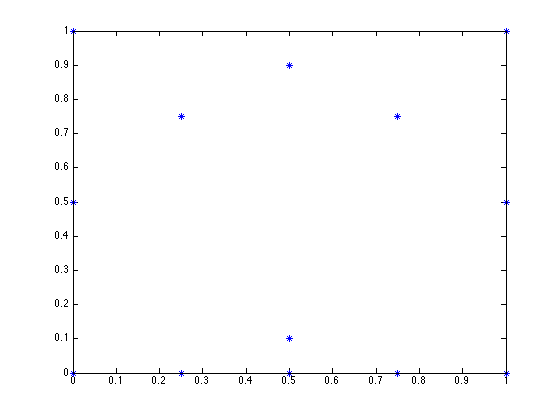
\includegraphics[scale=.5]{inicial1.png}
\caption{Distribución inicial de centros.}
\end{center}
\end{figure}
\begin{table}[H]
\caption{Resultados readaptando el parámetro de forma.}
\begin{center}
\begin{tabular}{|c|c|c|c|c|c|c|}
\hline
\ Tol & ECM & N & $D_{min}$ & Cond & $\epsilon$ & iter \\
\hline
\ $10^{-3}$ & 7.1902e-03 & 1291 & 1.5625e-02 & 4.7857e+12 & 6.4 & 6\\
\ $10^{-5}$ & 8.9364e-04 & 370 & 3.1250e-02& 3.2140e+11 & 3.2 & 5 \\
\ $10^{-7}$& 4.5348e-04 & 108 & 6.2500e-02 & 8.3501e+10 & 1.6 & 4 \\
\hline
\end{tabular}
\end{center}
\end{table}

\begin{figure}[H]
\begin{center}
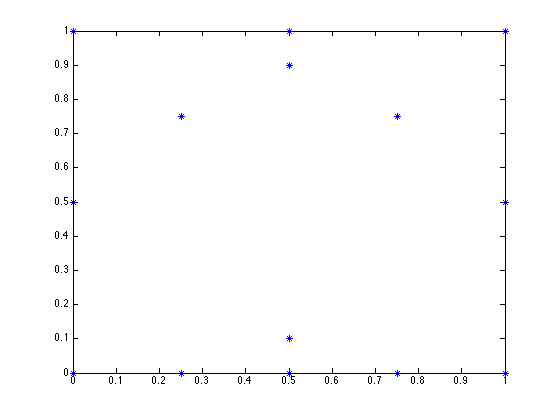
\includegraphics[scale=.4]{edp1_tol1.png}
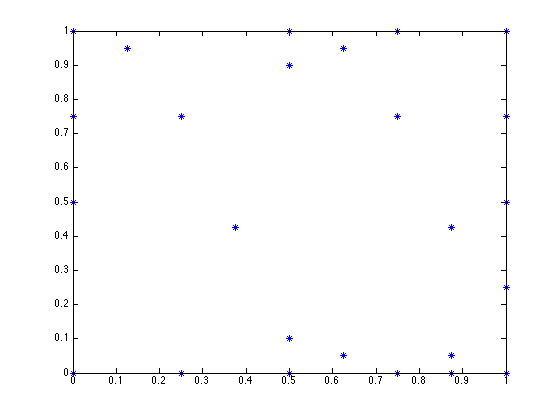
\includegraphics[scale=.4]{edp1_tol2.png}
\linebreak
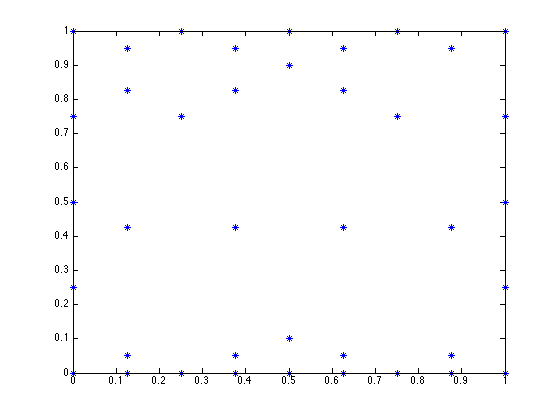
\includegraphics[scale=.4]{edp1_tol3.png}
\caption{Distribución final de los  centros  con toleracias $10^{-3}$, $10^{-5}$, y $10^{-7}$.}
\end{center}
\end{figure}





\begin{table}[H]
\caption{Resultados sin readaptar el parámetro de forma.}
\begin{center}
\begin{tabular}{|c|c|c|c|c|c|c|}
\hline
\ Tol & ECM & N & $D_{min}$ & Cond & $\epsilon$ & iter \\
\hline
\ $10^{-3}$ & 2.7199e-04& 39 & 5.0000e-02 &8.0904e+14 &0.4& 3  \\
\ $10^{-5}$ & 1.4542e-04& 1398 & 6.2500e-03 & 1.2472e+20 & 0.4 &6\\
\ $10^{-7}$ & 7.7231e-05 & 370 & 1.2500e-02& 5.0341e+19& 0.4 & 5\\
\hline
\end{tabular}
\end{center}
\end{table}

\begin{figure}[H]
\begin{center}
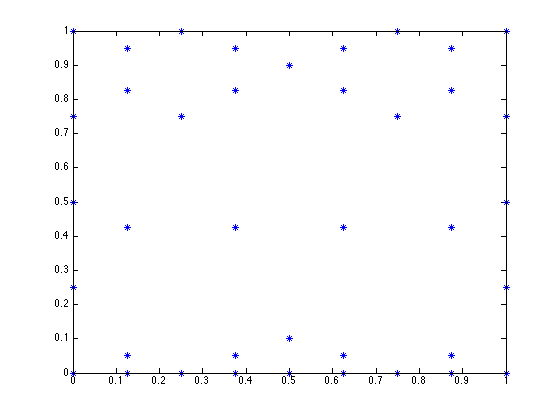
\includegraphics[scale=.4]{edp1_tol1_2.png}
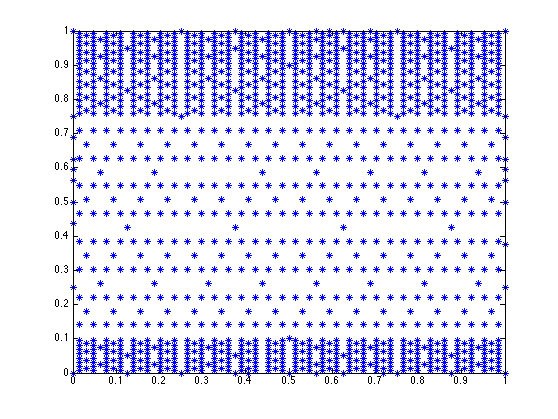
\includegraphics[scale=.4]{edp1_tol2_2.png}
\linebreak
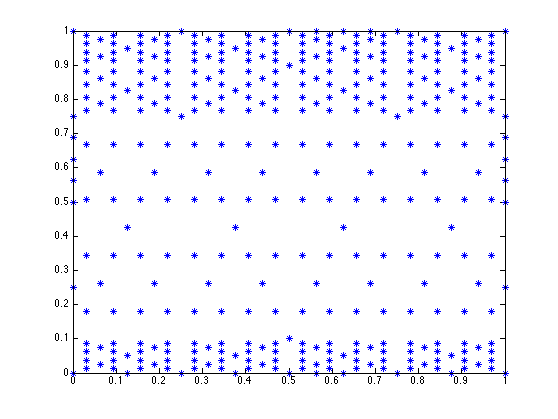
\includegraphics[scale=.4]{edp1_tol3_2.png}
\caption{Distribución final de los  centros  con toleracias $10^{-3}$, $10^{-5}$, y $10^{-7}$.}
\end{center}
\end{figure}
 \newpage
\textbf{Segundo ejemplo: edp 3}
\begin{figure}[H]
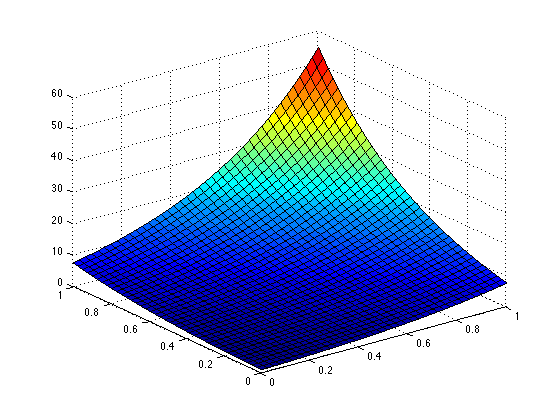
\includegraphics[scale=.45]{edp3.png}
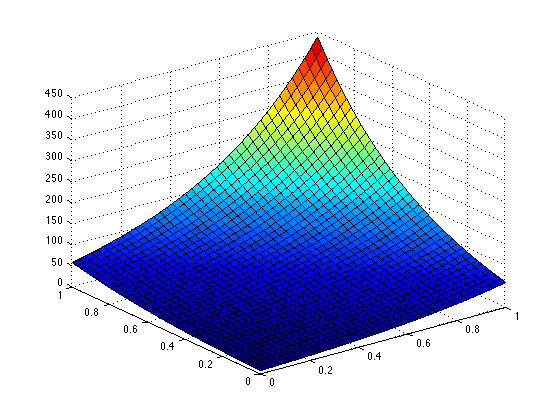
\includegraphics[scale=.45]{Ledp3.png}
\caption{Solución de la primera EDP y operador aplicado a la solución.}
\end{figure}

Distribución inicial de centros: 
\begin{figure}[H]
\begin{center}
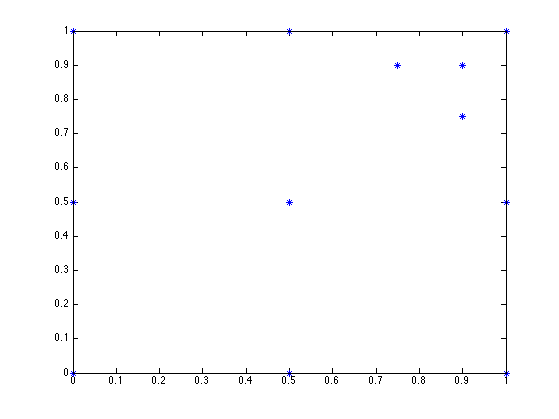
\includegraphics[scale=.5]{inicial2.png}
\caption{Distribución inicial de centros.}
\end{center}
\end{figure}

\begin{figure}[H]
\begin{center}
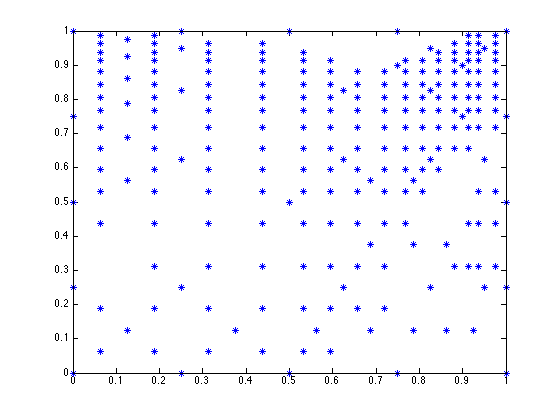
\includegraphics[scale=.4]{edp3_tol1_2.png}
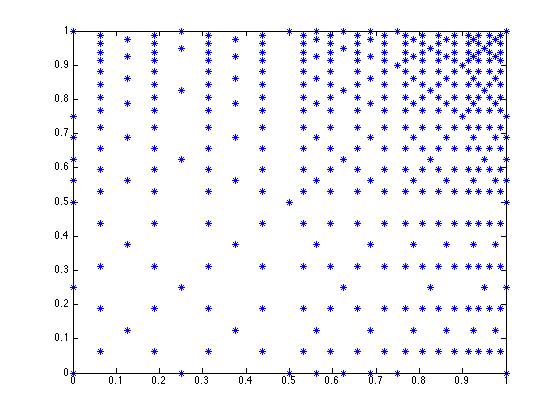
\includegraphics[scale=.4]{edp3_tol2_2.png}
\caption{Distribución final de los  centros  con toleracias $10^{-1}$, y $10^{-2}$.}
\end{center}
\end{figure}


\begin{table}[H]
\caption{Resultados sin readaptar el parámetro de forma.}
\begin{center}
\begin{tabular}{|c|c|c|c|c|c|c|}
\hline
\ Tol & ECM & N & $D_{min}$ & Cond & $\epsilon$ & iter \\
\hline
\ $10^{-1}$ & 1.4903e-03& 236& 1.2500e-02& 4.7954e+18& 1& 5\\
\ $10^{-2}$ & 1.8734e-02& 368& 1.2500e-02&2.4877e+19& 1&5\\
\hline
\end{tabular}
\end{center}
\end{table}

\textbf{Ejemplo del desplazamiento de los puntos de colocación y refinamiento de la rejilla}
\begin{figure}[H]
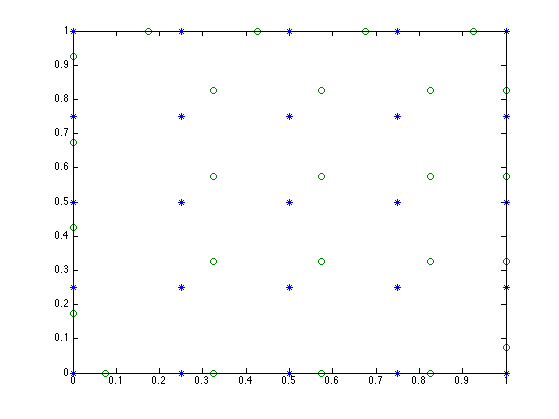
\includegraphics[scale=.4]{desplazamiento.png}
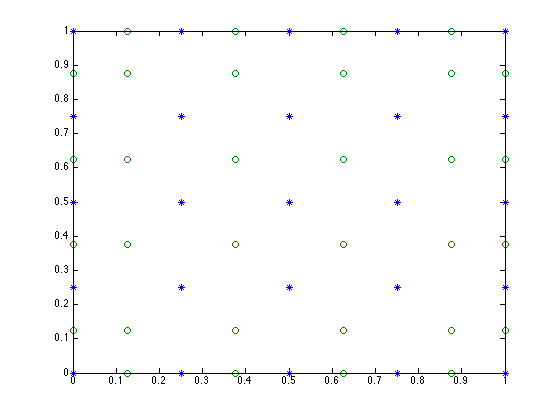
\includegraphics[scale=.4]{refinamiento.png}
\caption{Desplazamiento de los puntos de colocación + Refinamiento de la rejilla de puntos de colocación. }
\end{figure}


\end{document}

